\chapter{Technical Details}
\label{chap:implementation}

\section{Virtualization}
The most important concept of cloud computing and therefore also for IaaS systems is virtualization. Nowadays every cloud computing system is virtualized. This means that all the user's cloud computing applications run in virtual machines. In the case of IaaS systems the user buys a VM and can install whatever system he likes on it \cite{Arzuaga_2010}. 

Virtualization brings many advantages. A lot of crucial concepts of cloud computing are a lot easier with virtualized systems. On example is load balancing: Virtual machines can be copied and can be migrated on other physical machines without any problems - Figure \ref{fig:virtualization_live_migration} illustrates this graphically. The following section will give you a greater insight into load balancing strategies \cite{Arzuaga_2010}.

\begin{figure}
	\centering
		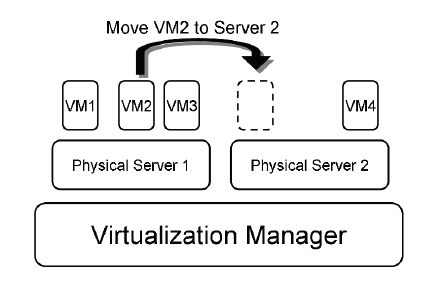
\includegraphics{virtualization}
	\caption{Virtualization and Live VM Migration in Cloud Computing Systems \cite{Arzuaga_2010}}
	\label{fig:virtualization_live_migration}
\end{figure}

\section{Load Balancing}
\label{sec:load_balancing}
As mentioned in the previous section, the applications on cloud computing systems run in virtual machines, and these VMs run in physical machines. Furthermore, there is a huge variation on the load (or resource needs) on the applications, therefore if there run too many applications (or VMs) on one physical machine it may get overloaded. This is why one needs load balancing. Load balancing should avoid that the physical machines have to handle more resources than they can offer. These resources can be CPU, RAM or storage space. If there run too many VMs on one physical machine this can mean a tremendous slow down of the VMs running on it. But slow VMs and applications are not the only problems, that bad load balancing would cause. If a application does not have sufficient resources, often the Service Level Agreement (SLA) is violated. A SLA is the agreement between customer and provider that guarantees certain parameters like performance and availability. A violation can mean that the cloud computing provider may have to give discount because of the violation or the customer decides to change to another cloud computing provider. As you can see good load balancing is crucial in the field of cloud computing \cite{Chen_2014}. 

\subsection{Load Balancing Algorithms}
There are many approaches on how load balancing algorithms should work, but they all have something in common: the input and the output. Every algorithm has to watch over the states of the physical and virtual machines and has to decide if a VM gets moved from. Furthermore, it has to decide which VM has to be migrated to which physical machine \cite{Chen_2014}.

Many common load balancing algorithms are based on the current states of the PMs and VMs. They therefore are called "reactive" algorithms. This means that when the resource utilization on a certain PM reaches a certain threshold, a VM gets migrated to another PM. This algorithm is rather easy to implement, as it only has to watch the current resource utilization at the physical machines, but the disadvantages are that it only considers the current state of the system and that when a the threshold is reached most often, an imbalance situation is yet the case. Furthermore, it cannot guarantee a long-term balance situation, as it only acts on the parameters known at that point of time \cite{Arzuaga_2010,Chen_2014}.

Other algorithms are based on a "proactive" approach. In these algorithms the physical machines try to predict the resource demand of the VMs running on them and if in the near future there would be a overload they migrate a VM to another physical machine which predicts a lower resource utilization. This has the advantage that if the algorithm works as desired and the estimates on the resource demands of the VMs are approximately correct, there won't be any more overloads, because the algorithm would predict correct and migrate the VMs before the physical machine is overloaded. Usually the proactive approaches give better results than the earlier discussed reactive approach. But, however, there are also disadvantages. The first one is that the physical machine does under usual circumstances not know, which VM should be migrated to another PM. Furthermore, in the long run this approach also does not create a balanced state, because it only predicts a certain time span in the future. Finally, there have to be made a lot of calculations to predict the resource needs of the VMs (this is usually done by a Markov model), especially when there are a lot of VMs per physical machine. This often creates a big load just for the load balancing algorithm \cite{Beloglazov_2013,Chen_2014}.

\section{Resilience Planning}

\section{Backup Strategies}

\section{Monitoring}
Monitoring is an essential part for deployed systems for both,  dedicated hardware structures and cloud computing systems. It enables to discover and analyze failure, bad configuration, performance bottle necks and many other issues that are important parts of software maintenance. Cloud computing systems are made to be highly scaleable and elastic. But these two characteristics make it hard to monitor cloud computing systems as monitoring of high scaling systems requires to collect, store and analyze a lot of data in real time, which can be computationally highly expensive. Furthermore, the high elasticity shows an extra challenge, as the whole environment can change in a very short period of time in modern clouds \cite{Ward_2014}.

\subsection{Common Architectures}
The most important architectures that are typical for monitoring distributed systems are:

\begin{itemize}
	\item Flat Pull Model: A central server polls all the machines he should monitor according to a schedule when machines join and leave.
	\item Hierarchical Pull Model: Monitoring servers poll a subset of all the servers which should be monitored. A central server then polls the monitoring servers.
	\item Hierarchical Push Model: The server themselves push information to a monitoring server which is assigned to them and the monitoring servers collect that information from their machines and push it to a central server \cite{Ward_2014}.
\end{itemize}

However, the just mentioned models for monitoring are modeled for grid and cluster computing. They are not always optimal for cloud computing systems as virtual machines can dynamically be added and removed and this creates the need for other approaches \cite{Ward_2014, He_2010}. 

In 2010, Huang \cite{He_2010} proposed a monitoring system he called "Push and Pull", which should combine the advantages of the push and pull model. In current pull systems, the consumers pull information from the producers in a certain interval. This approach is efficient but lacks in consistency. If the interval is too big, data is lost, but if the interval is too small it is inefficient. In push systems on the other hand producers tell the consumers changes whenever the changes are greater than a threshold. This can produce good performance depending on the threshold and all data changes are monitored, but if the threshold is too small, too much information is transmitted and this leads to inefficiency. 